\documentclass[preview]{standalone}
\usepackage{helvet}
\renewcommand{\familydefault}{\sfdefault}
\usepackage{ulem}

%\usepackage{floatrow}
\usepackage{graphicx}
\graphicspath{{./otherFigures/}}
\usepackage{caption}
\usepackage[label font=bf,labelformat=simple, position = top, justification=RaggedRight,singlelinecheck=false]{subfig}
\newdimen\figrasterwd
\figrasterwd\textwidth
%\floatsetup[figure]{style=plain,subcapbesideposition=top}
\newsubfloat{figure}


\begin{document}
%\begin{figure}
%\centering
  %\parbox{.95\figrasterwd}{
    %\parbox{.6\hsize}{%
      %\subfloat[][]{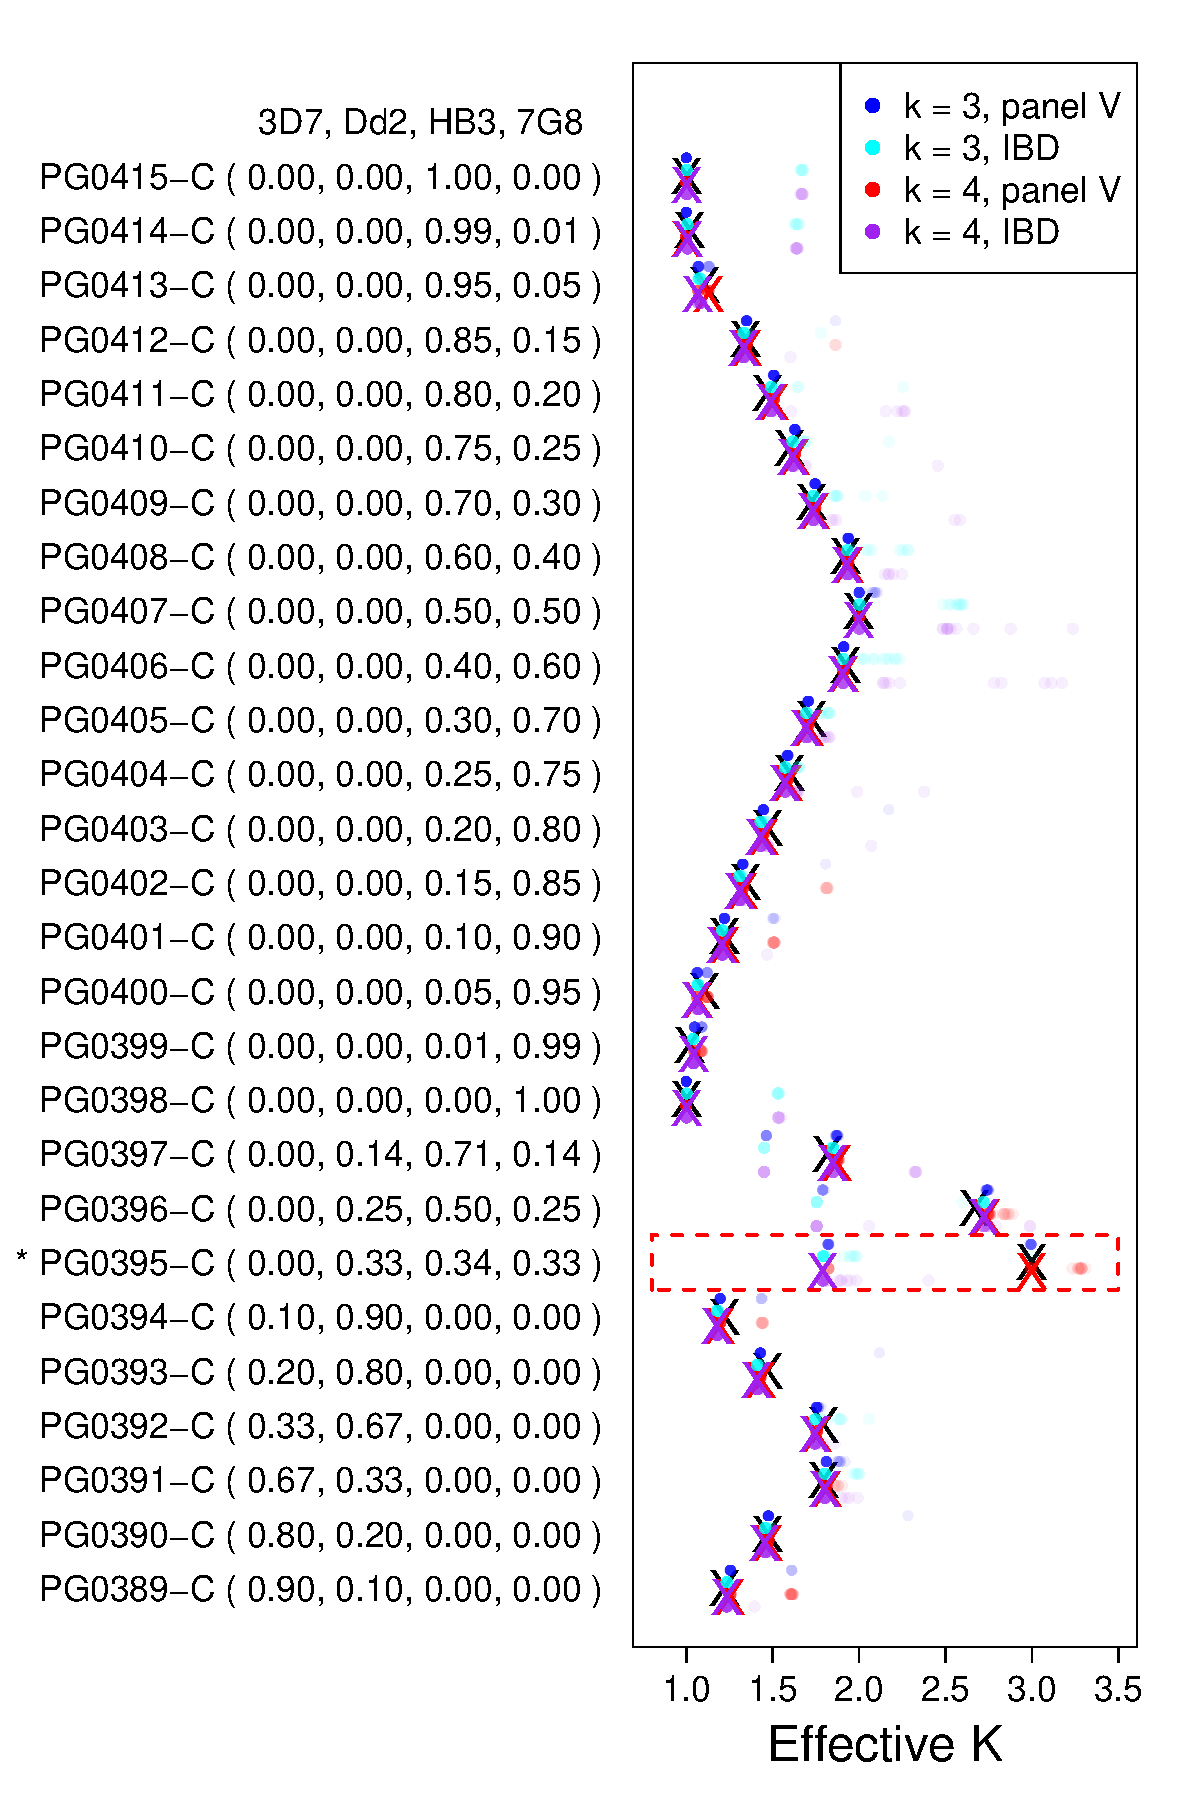
\includegraphics[width=\hsize]{eff_k_both.pdf}}
    %}
    %\hskip1em
    %\parbox{.4\hsize}{%
      %\subfloat[][]{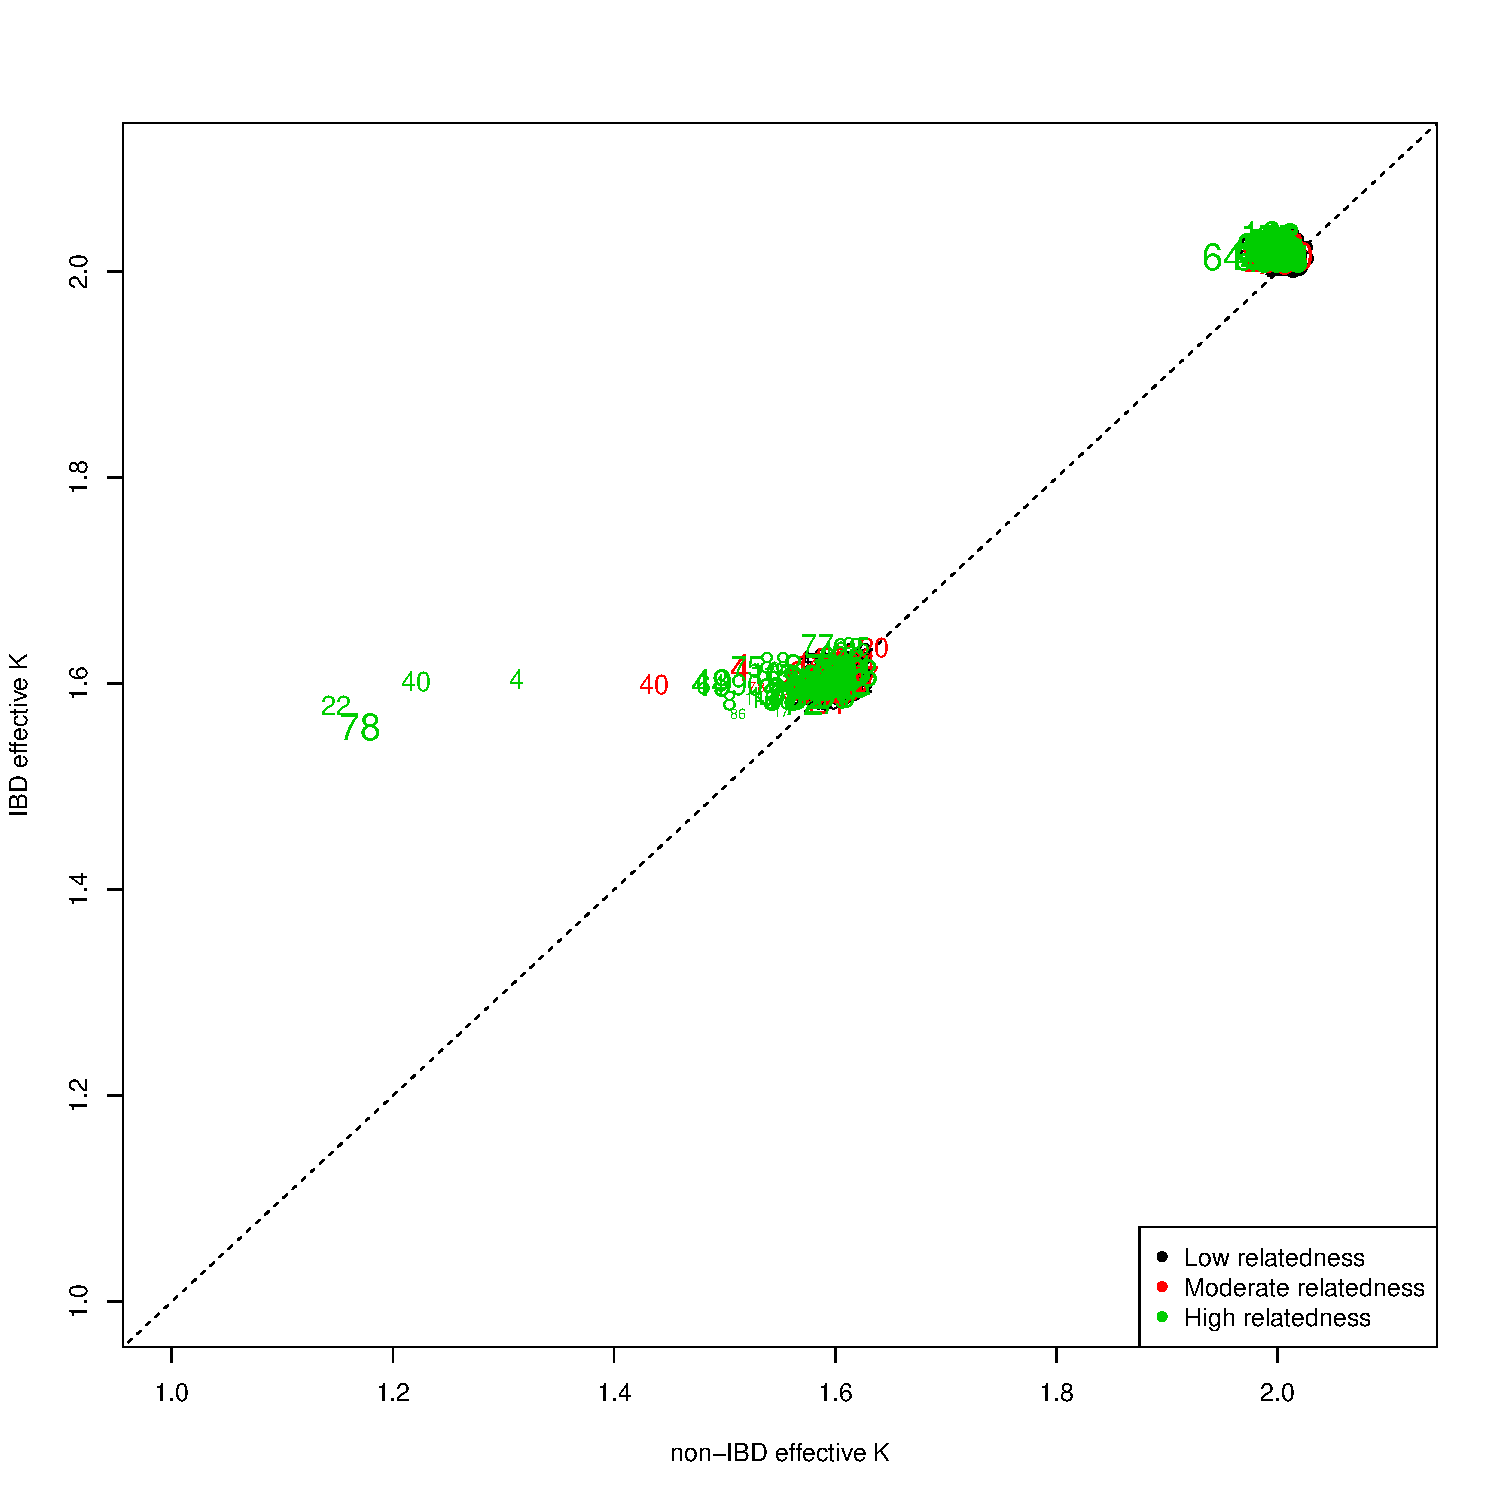
\includegraphics[width=\hsize]{diagnositicPlot_of_effK_final.pdf}}
      %\\
      %%\vskip1em
      %\subfloat[][]{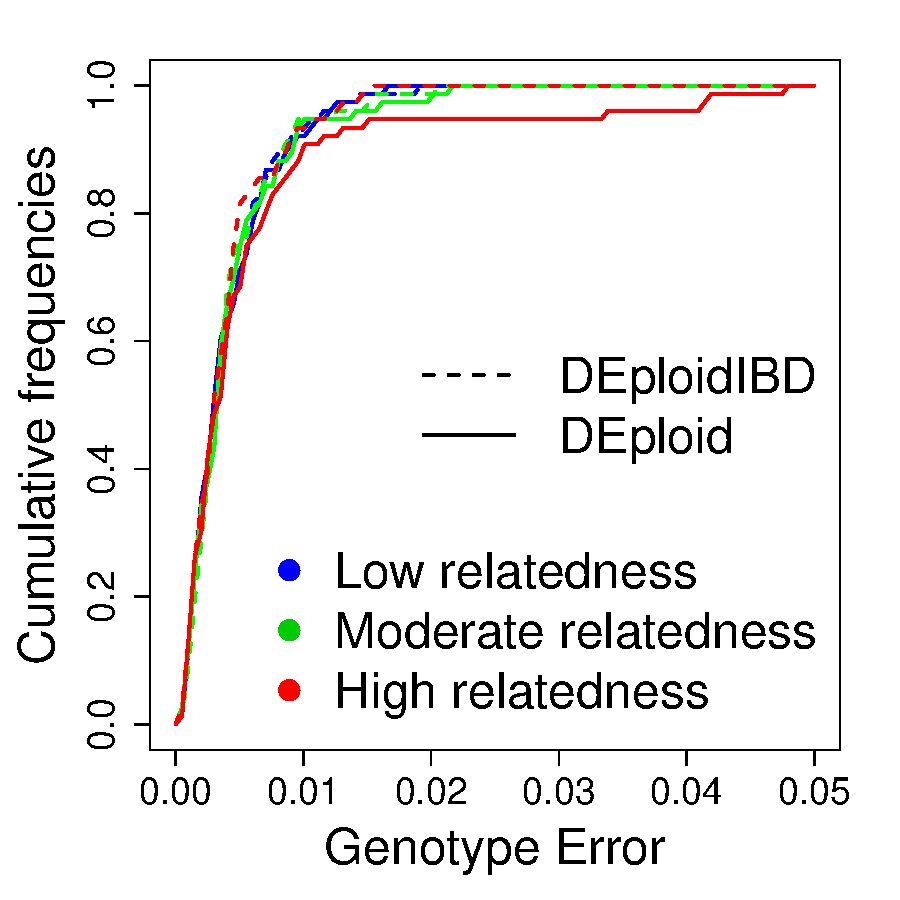
\includegraphics[width=\hsize]{genotype_error_ecdf.pdf}}
    %}
  %}
%\end{figure}
\begin{figure}
\centering
  \subfloat[][]{\includegraphics[width=0.33\textwidth]{diagnositicPlot_of_effK_final_newlook.pdf}}
  \subfloat[][]{\includegraphics[width=0.33\textwidth]{ForFig2.pdf}}
  \subfloat[][]{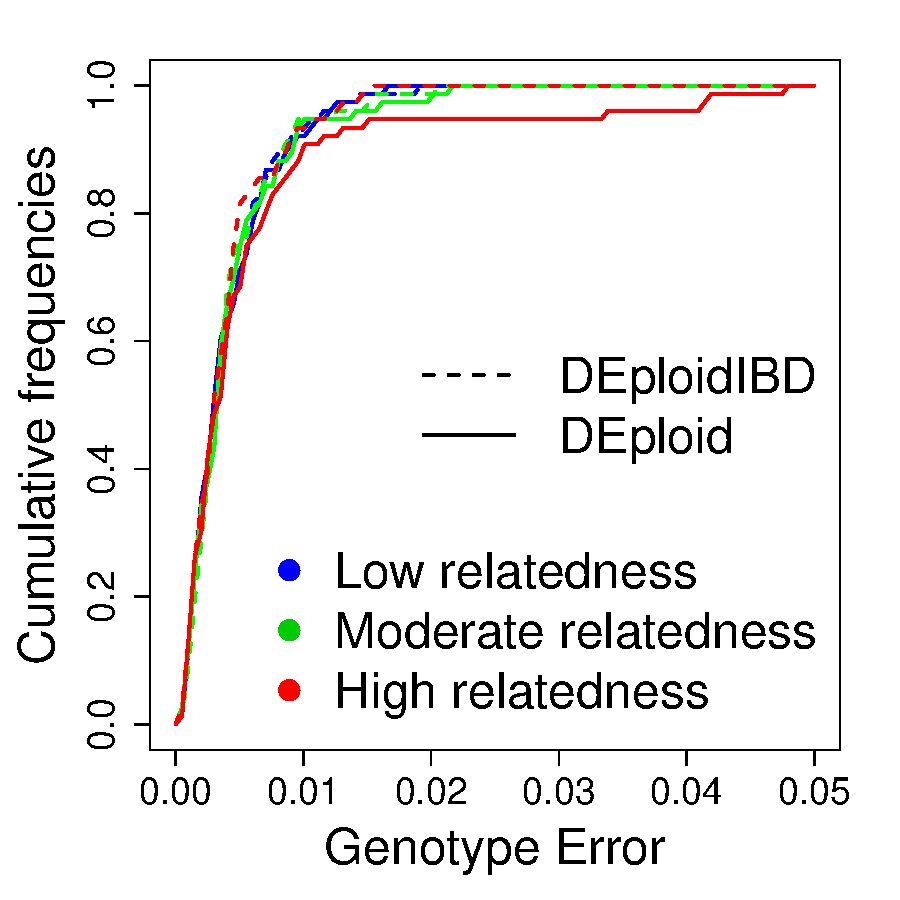
\includegraphics[width=0.33\textwidth]{genotype_error_ecdf.pdf}}
\end{figure}
\end{document}

